% Options for packages loaded elsewhere
\PassOptionsToPackage{unicode}{hyperref}
\PassOptionsToPackage{hyphens}{url}
%
\documentclass[
]{book}
\usepackage{amsmath,amssymb}
\usepackage{iftex}
\ifPDFTeX
  \usepackage[T1]{fontenc}
  \usepackage[utf8]{inputenc}
  \usepackage{textcomp} % provide euro and other symbols
\else % if luatex or xetex
  \usepackage{unicode-math} % this also loads fontspec
  \defaultfontfeatures{Scale=MatchLowercase}
  \defaultfontfeatures[\rmfamily]{Ligatures=TeX,Scale=1}
\fi
\usepackage{lmodern}
\ifPDFTeX\else
  % xetex/luatex font selection
\fi
% Use upquote if available, for straight quotes in verbatim environments
\IfFileExists{upquote.sty}{\usepackage{upquote}}{}
\IfFileExists{microtype.sty}{% use microtype if available
  \usepackage[]{microtype}
  \UseMicrotypeSet[protrusion]{basicmath} % disable protrusion for tt fonts
}{}
\makeatletter
\@ifundefined{KOMAClassName}{% if non-KOMA class
  \IfFileExists{parskip.sty}{%
    \usepackage{parskip}
  }{% else
    \setlength{\parindent}{0pt}
    \setlength{\parskip}{6pt plus 2pt minus 1pt}}
}{% if KOMA class
  \KOMAoptions{parskip=half}}
\makeatother
\usepackage{xcolor}
\usepackage{longtable,booktabs,array}
\usepackage{calc} % for calculating minipage widths
% Correct order of tables after \paragraph or \subparagraph
\usepackage{etoolbox}
\makeatletter
\patchcmd\longtable{\par}{\if@noskipsec\mbox{}\fi\par}{}{}
\makeatother
% Allow footnotes in longtable head/foot
\IfFileExists{footnotehyper.sty}{\usepackage{footnotehyper}}{\usepackage{footnote}}
\makesavenoteenv{longtable}
\usepackage{graphicx}
\makeatletter
\def\maxwidth{\ifdim\Gin@nat@width>\linewidth\linewidth\else\Gin@nat@width\fi}
\def\maxheight{\ifdim\Gin@nat@height>\textheight\textheight\else\Gin@nat@height\fi}
\makeatother
% Scale images if necessary, so that they will not overflow the page
% margins by default, and it is still possible to overwrite the defaults
% using explicit options in \includegraphics[width, height, ...]{}
\setkeys{Gin}{width=\maxwidth,height=\maxheight,keepaspectratio}
% Set default figure placement to htbp
\makeatletter
\def\fps@figure{htbp}
\makeatother
\setlength{\emergencystretch}{3em} % prevent overfull lines
\providecommand{\tightlist}{%
  \setlength{\itemsep}{0pt}\setlength{\parskip}{0pt}}
\setcounter{secnumdepth}{5}
\usepackage{booktabs}
\ifLuaTeX
  \usepackage{selnolig}  % disable illegal ligatures
\fi
\usepackage[]{natbib}
\bibliographystyle{apalike}
\IfFileExists{bookmark.sty}{\usepackage{bookmark}}{\usepackage{hyperref}}
\IfFileExists{xurl.sty}{\usepackage{xurl}}{} % add URL line breaks if available
\urlstyle{same}
\hypersetup{
  pdftitle={Hidden Markov Models \& their Applications to Statistical Genetics},
  pdfauthor={Sofia Barragan, Spring 2021, Macalester College},
  hidelinks,
  pdfcreator={LaTeX via pandoc}}

\title{Hidden Markov Models \& their Applications to Statistical Genetics}
\author{Sofia Barragan, Spring 2021, Macalester College}
\date{}

\begin{document}
\maketitle

{
\setcounter{tocdepth}{1}
\tableofcontents
}
\hypertarget{welcome}{%
\chapter*{Welcome}\label{welcome}}
\addcontentsline{toc}{chapter}{Welcome}

This bookdown on discrete Hidden Markov Models \& their applications to statistical genetics is my capstone! I made this for my Mathematical Statistics course taught by \href{http://kegrinde.github.io}{Kelsey Grinde}. Big thanks to her for her guidance and help.

Content was written and gathered by \href{https://www.sofiabarragan.com}{Sofia Barragan} with appropriate citations for print materials. Wherever possible, I try to provide direct link citations for any digital materials or resources.

Embedded Youtube videos are under the sole ownership of their linked creator.

\textbf{Note:} This is a very brief primer \& I assume minimal mathematical background.


\includegraphics{images/cc_license_button.png}

This work is licensed under a \href{https://creativecommons.org/licenses/by-nc-sa/4.0/}{Creative Commons Attribution-NonCommercial-ShareAlike 4.0 International License}.

\hypertarget{mathematical-intuition}{%
\chapter{Mathematical Intuition}\label{mathematical-intuition}}

Markov Chains are cool! Hidden Markov Models are also cool, but require more preparation! In this section, we'll go through conditional probabilities \& set up the basis to study Hidden Markov Models by getting comfortable with chains first.

\hfill\break

\begin{center}\rule{0.5\linewidth}{0.5pt}\end{center}

\hypertarget{conditional-probability-bayes-rule}{%
\section{Conditional Probability \& Bayes Rule}\label{conditional-probability-bayes-rule}}

\hypertarget{basic-concepts}{%
\subsection*{Basic Concepts}\label{basic-concepts}}
\addcontentsline{toc}{subsection}{Basic Concepts}

Probability, as a field, formalizes how we predict events with some equally beautiful \& ugly notation, intuitive concepts, and complex mathematical principles. But the premise is simple: by ascribing a numeric value to the outcomes of an event, we can abstract the real world and study it with math.

The process of ascribing numeric values to the outcome of an event is called mapping \& by mapping all possible probabilities of an event's outcomes, we create a \textbf{random variable}.

\begin{quote}
\textbf{NOTE:} This can be confusing! The ``random'' part of the word doesn't mean all outcomes have an equal chance of happening; really, it means that within an event, there are multiple possible outcomes.
\end{quote}

\hfill\break

\textbf{Example: Weather \& Temperature}

Let's say that the weather is the event, \(W\), whose only \textbf{outcomes} are sunny (\(w_s\)), rainy (\(w_r\)) or cloudy(\(w_c\)).
By mapping numeric values (e.g., probabilities) to the outcomes, we can turn \(W\) into a random variable. Below, we list all mappings in the \textbf{probability mass function}, \(p_{(W)}(w)\).

\begin{align*} 
p_{(W)}(w)  &= \begin{cases}
    0.5, & \text{for } w_s \\
    0.2, & \text{for } w_r \\
    0.3, & \text{for } w_c \\
    0.0, & \text{otherwise}
\end{cases}
\end{align*}

\hfill\break

\begin{quote}
\textbf{NOTE:} The sub-probability of \emph{all} probability mass functions must sum to 1.
\end{quote}

\hfill\break

Now, let's see that the daily temperature (F°) is the event \(T\). Normally, we could say that \(T\) follows a normal distribution with \(\mu = 75 \textbf{ F°}\) and \(\sigma^2 = 625 \textbf{ F°}\), since its a continuous variable. So, \(T \sim N(75, 625)\) and would look something like this

\begin{center}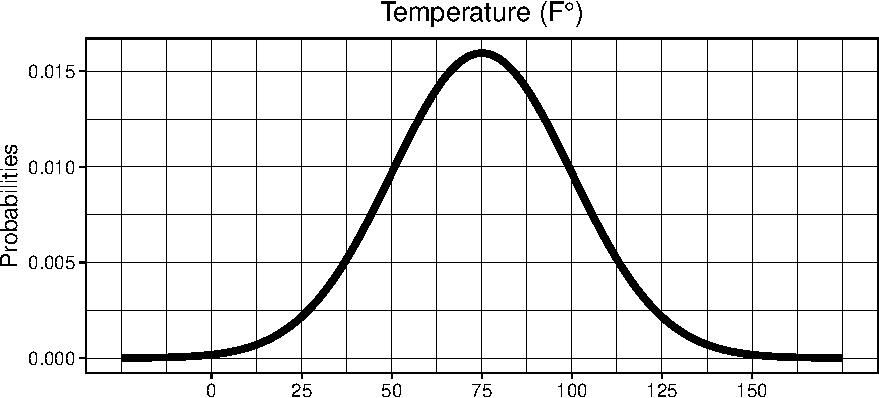
\includegraphics{455_HMM_files/figure-latex/unnamed-chunk-3-1} \end{center}

\hfill\break

Instead, let's say that \(T\) is a discrete random variable whose only potential outcomes are cold (\(t_c\)), fresh (\(t_n\)), or hot (\(t_h\)). Then, \(T\) has the probability mass function

\begin{align*} 
p_{(T)}(t)  &= \begin{cases}
    0.155, & \text{for } t_c \\
    0.5, & \text{for } t_f \\
    0.345, & \text{for } t_h \\
    0.0, & \text{otherwise}
\end{cases}
\end{align*}

\hfill\break

Below are two graphs summarizing what we know so far about \(W\) and \(T\)

\begin{center}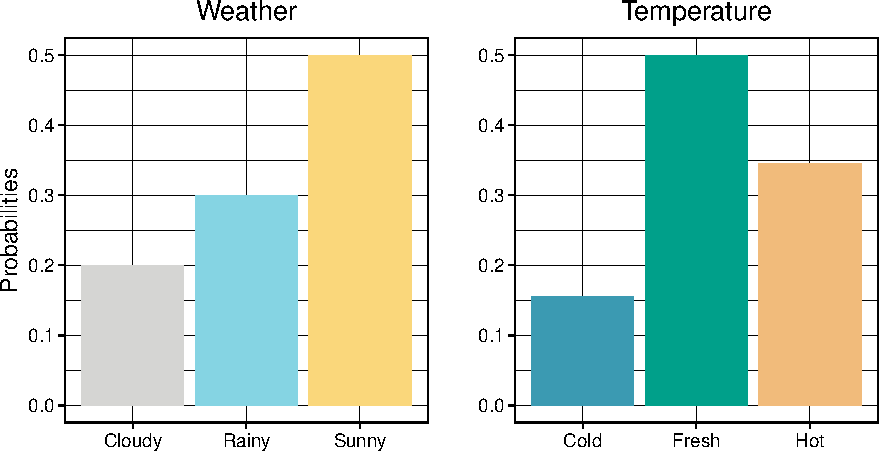
\includegraphics{455_HMM_files/figure-latex/unnamed-chunk-6-1} \end{center}

But what happens if the weather depends on the temperature?

\hfill\break
\hfill\break

\hypertarget{conditional-probabilities}{%
\subsection*{Conditional Probabilities}\label{conditional-probabilities}}
\addcontentsline{toc}{subsection}{Conditional Probabilities}

Let's study the two arbitrary events \(A\), \(B\) \& learn some definitions about probability.

\textbf{Conditional Probability:}
The conditional probabilities of \(A\)'s, given \(B\) and \(B\), given \(A\) are written below.
\[P(A \mid B) \hspace{1 in}P(B \mid A)\]\\

\textbf{Independence:}
We say that the two events, \(A\) \& \(B\) are independent if the conditional probabilities provide us no new-information about either event. So,

\[P(A \mid B) = P(A) \hspace{1 in}P(B \mid A) = P(B)\]\\

\textbf{Joint Probability:}
The probability of two events, \(A\) \& \(B\) happening at the same time is called a \textbf{joint probability} and is typically denoted by \(P(A\cap B)\). It is calculated below.

\begin{align*} 
P(A\cap B) &= P(A \mid B) \cdot P(B)\\
&= P(A) \cdot P(B) && \text{if independent}
\end{align*}

\hfill\break
\hfill\break

It's generally true that the weather on a particular day, depends on the temperature. This implies that \(W\) and \(T\) are conditional events with conditional probabilities. So,

\[P(W\mid T) \neq P(W)\]

\hypertarget{bayes-rule-lotp}{%
\subsection*{Bayes' Rule \& LOTP}\label{bayes-rule-lotp}}
\addcontentsline{toc}{subsection}{Bayes' Rule \& LOTP}

Conceived by Reverend Thomas Bayes in the 18th Century, posthumously published by his friend Richard Price, and then formalized into an equation by Pierre-Simon Laplace, Bayes' Rule is a cornerstone equation in modern statistics \& probability\footnote{\url{https://www.bayesrulesbook.com/chapter-1.html\#a-quick-history-lesson}}. I've written Bayes Rule below\footnote{\url{https://www.bayesrulesbook.com/chapter-2.html}}

\[P(A \mid B) = \frac{P(A \cap B)}{P(B)}=\frac{P(A)\cdot P(B \mid A)}{P(B)}\]

\begin{quote}
\textbf{NOTE}: Above you'll notice that we're looking at the probability of \(A\) \& \(B\), divided by the probability of \(B\). We are dividing by \(P(B)\) to normalize \& isolate the probability of \(A\), under the conditions we observe \(B\).
\end{quote}

\begin{quote}
\textbf{Quick Check:} If \(A\) \& \(B\) are independent, how would you further simplify the numerator of Bayes' Rule?
\end{quote}

The denominator of Bayes' Rule, \(P(B)\) is called the \textbf{marginal probability} of \(B\).

The marginal probability can either be

\begin{itemize}
\tightlist
\item
  given
\item
  computed with the \textbf{law of total probability} or (\textbf{LOTP}).
\end{itemize}

\textbf{LOTP} states that

\begin{align*}
P(B) = \sum_{i=1}^n P(B \cap A_i) &= P(B \cap A_1) + P(B\cap A_2) + \dots + P(B\cap A_n) \\
&= P(B \mid A_1)P(A_1) + P(B\mid A_2)P(A_2) + \dots + P(B\mid A_n)P(A_n) \\
\end{align*}

\begin{quote}
\textbf{Note:} Looks scary! Really it's like calculating the probability of \(B\) in each subcategory of \(A\), multiplying by the probability of that sub-\(A\), then adding it all together.
\end{quote}

\hfill\break

\begin{center}\rule{0.5\linewidth}{0.5pt}\end{center}

\hypertarget{markov-chains}{%
\section{Markov Chains}\label{markov-chains}}

\textbf{Stochastic processes} are events that have some element of randomness in their outcomes. The amount of `randomness' \& the type of events can vary depending on the context. In turn, studying the properties of stochastic processes often requires many different techniques which go well beyond the boundaries of statistics. And with a litany of applications across so many domains of knowledge, studying stochastic processes also involves many techniques from Physics, Linguistics, Sociology, Public Health, Geography \& more.

\begin{quote}
\textbf{Note:} There is \emph{some} nuance in the language we use to describe randomness, probabilistic, and stochastic, but it is murky. So, for now, let's stick with the above definition \& enjoy some interchangeability between random, stochastic, and probabilistic.
\end{quote}

So, this section will only be a tiny snippet of the wide topics covered in studying stochastic processes.

\hypertarget{intuition}{%
\subsection*{Intuition}\label{intuition}}
\addcontentsline{toc}{subsection}{Intuition}

Markov chains are a subclass of stochastic processes that describe partially random events occurring in succession, typically in succession. We will formalize this definition soon, but for now, let's talk about the weather.

\textbf{Example: Weather}

Let's ignore the fact that temperature determines weather. Instead, let's assume that we can compute the probability of tomorrow's weather by only looking at today's. This results in three important ideas:

\begin{itemize}
\tightlist
\item
  General weather patterns before today are irrelevant when predicting tomorrow's weather. This is an example of a Markov process, more specifically a Markov Chain.
\item
  The outcomes of the weather are rainy, sunny, or cloudy. These are examples of states.
\item
  The probability of tomorrow's weather depends on whether it was rainy, sunny, or cloudy to day. Meaning there are probabilities associated with tomorrow's events, strictly defined by today's. These are examples of transition probabilities.
\end{itemize}

Let's be rigorous now!

\hypertarget{mathematical-definitions}{%
\subsection*{Mathematical Definitions}\label{mathematical-definitions}}
\addcontentsline{toc}{subsection}{Mathematical Definitions}

Let \(X_i = X_1, \dots, X_{n-1}, X_n\) be a collection of \(n\) successively indexed events.

The discrete \(X_i\) are a \textbf{Markov Chain} if

\begin{itemize}
\tightlist
\item
  They exhibit a \textbf{Markov Property}.

  \begin{itemize}
  \tightlist
  \item
    Where the probability of some new or predicted event \(X_{n+1}=x_{n+1}\) is
  \end{itemize}
\end{itemize}

\[P(X_{n+1} = x_{n+1} \mid X_1 = x_1, \dots,  X_{n-1}= x_{n-1}, X_n= x_{n}) = P(X_{n+1} = x_{n+1} \mid X_n = x_n)\]

\begin{quote}
\textbf{NOTE:} This is similar to the conditional probability of independent events! But instead we specify that prior events \(X_1,\dots X_{n-1}\) are independent of the outcome of \(X_{n+1}\), but \(X_{n}\) is not.
\end{quote}

\hfill\break

\begin{itemize}
\tightlist
\item
  There is some countable set of outcomes called the \textbf{State Space} which contains every possible outcome or \textbf{State}

  \begin{itemize}
  \tightlist
  \item
    The outcomes \(x_1, \dots, x_{n-1}, x_{n}, x_{n+1}\) are all common elements of the state space, \(\mathbb{S}\).
  \end{itemize}
\end{itemize}

\begin{quote}
\textbf{NOTE:} This may seem complicated, but this means we can define what are possible and impossible outcomes.
\end{quote}

\hfill\break

\begin{itemize}
\tightlist
\item
  The probability of changing states is a \textbf{Transition Probability} and if we were to write them out for each \emph{state}, they would sum to \(1\).

  \begin{itemize}
  \tightlist
  \item
    Transition Probabilities sum to 1 because they cumulatively define the \emph{probability mass function} of the transition from each state to another.
  \item
    These probabilities can be placed in a \textbf{Transition Matrix} where the columns indicate a next state \& the rows indicate the current state.
  \end{itemize}
\end{itemize}

\begin{quote}
\textbf{NOTE:} The above definitions were cumulatively drawn from the following sources \footnote{Lay, David C. 2012. ``Applications to Markov Chains.'' In Linear Algebra and Its Applications, 4th ed., 253--62. Boston: Pearson College Division.} \footnote{\url{https://setosa.io/ev/markov-chains/}}
\end{quote}

\hfill\break

\hypertarget{visualizations}{%
\subsection*{Visualizations}\label{visualizations}}
\addcontentsline{toc}{subsection}{Visualizations}

\textbf{Weather Graphs}

Below we've redefined our weather example as a Markov Chain, using our new definitions, and place it into a Weighted Directed Graph. Isn't she pretty! Note that the \emph{weights} on our arrows correspond to the transition probability associated with that change-arrow.

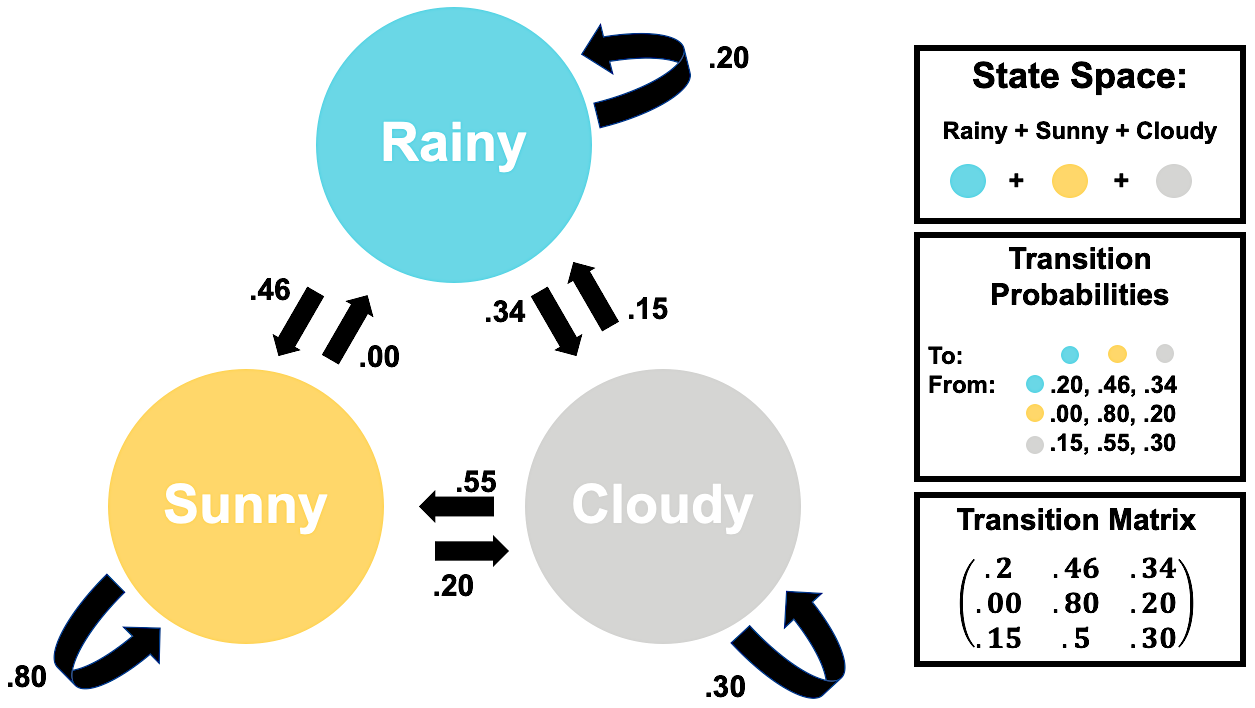
\includegraphics{images/HMM_Diagram_Intuition.png}

Also, check out that Transition Matrix! It's the first one you've looked at, but they can quickly get very complex.

\hfill\break

\textbf{Weather Animations}

To simulate how a Markov Chain of weather behaves, let's animate it!

In this visualization, there are 10 multicolored dots representing different arbitrary days colored by that particular day's weather. To see how Markov Chains evolve over 15 days, we shuffle them 15 times in a row according to our transition matrix

\begin{longtable}[]{@{}ccc@{}}
\toprule\noalign{}
Rainy & Sunny & Cloudy \\
\midrule\noalign{}
\endhead
\bottomrule\noalign{}
\endlastfoot
.20 & .46 & .34 \\
.00 & .80 & .20 \\
.15 & .50 & .30 \\
\end{longtable}

Written text describes the proportion of weather outcomes following simulation. That is, how many rainy, sunny, or cloudy days happen after a given shuffle.

Look at that! We converged on our initial probability distribution. That isn't necessarily true for all simulations, but it's true for this one.

\begin{quote}
\textbf{NOTE:} This Markov Chain visualization was designed by \href{https://willhipson.netlify.app}{Will Hipson}, a graduate student in Psychology at Carleton University. You can find links for reproduction at his page\footnote{\url{https://willhipson.netlify.app/post/markov-sim/markov_chain/}} or check out my GitHub to see my edits.
\end{quote}

\hfill\break

\begin{center}\rule{0.5\linewidth}{0.5pt}\end{center}

\hypertarget{conclusion}{%
\section{Conclusion}\label{conclusion}}

We've covered the necessary probability concepts. In the next section, we'll find out out how we can leverage Markov Chains to predict another set of variables, even when we can't see the outcomes of our chain. Prepare for bivariate distributions, many subscripts, and a lot of summation notation!

If you have any lingering questions, I've linked some great YouTube videos that may be helpful below.

\hypertarget{video-resources}{%
\section*{Video Resources}\label{video-resources}}
\addcontentsline{toc}{section}{Video Resources}

\textbf{Conditional Probability}

\textbf{Bayes Rule}

\textbf{Markov Chains}

\hypertarget{references}{%
\section*{References}\label{references}}
\addcontentsline{toc}{section}{References}

\hypertarget{frog-families-hmms}{%
\chapter{Frog Families \& HMMs}\label{frog-families-hmms}}

Previously, we wanted to study the weather. Let's up the stakes and now look at how the weather can determine whether or not a cute, infinitely reproducing, frog-family survives the month.

If you were a frog, you wouldn't be able to check the weather before leaving your tree hide-- you wouldn't even be able to read!-- but you do know that when a family member leaves for their daily hop, their chance of living depends on the weather. If the weather is

\begin{itemize}
\tightlist
\item
  \textbf{Sunny:} they would have a 10\% chance of living (and eating a nice bug) with a 90\% chance of dying.
\item
  \textbf{Cloudy:} they would have a 75\% chance of living (and eating a nice bug) with a 25\% chance of dying.
\item
  \textbf{Rainy:} they would have a 98\% chance of living (and eating a nice bug) with a 2\% chance of dying.
\end{itemize}

Since we, as non-frog statisticians, know that the weather is a Markov Chain, we can say the survival of this frog-family is actually a Hidden Markov Model. In the following sections, we will establish what that implies theoretically for us \& our frog family.

\hfill\break

\begin{center}\rule{0.5\linewidth}{0.5pt}\end{center}

\hypertarget{hidden-markov-models}{%
\section{Hidden Markov Models}\label{hidden-markov-models}}

Hidden Markov Models are another class of probabilistic models that model Markov processes whose outcomes cannot be directly observed, but their dependent observed events can be. Often, we're really interested in these unobserved events and predicting them, so we can work backward and use the observed ones\footnote{\url{https://www.nature.com/articles/nbt1004-1315\#citeas}}.

Intuitively, it's like using the shadow of an animal to guess what it is!

\begin{figure}
\hypertarget{id}{%
\centering
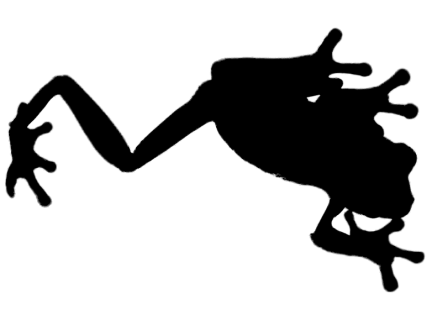
\includegraphics[width=0.5\textwidth,height=0.5\textheight]{images/frogshadow.png}
\caption{Fig 1. Frog Shadow Made by Author}\label{id}
}
\end{figure}

\hfill\break

\hypertarget{properties}{%
\subsection*{Properties}\label{properties}}
\addcontentsline{toc}{subsection}{Properties}

\textbf{Let}

\begin{itemize}
\tightlist
\item
  \(X_i = X_1=x_1, \dots, X_{n-1}=x_{n-1}, X_n =x_n\) be a collection of \(n\) successively indexed events.
\item
  \(Y_i = Y_1=y_1, \dots, Y_{n-1}=y_{n-1}, Y_n =y_n\) be a collection of \(n\) successively indexed observations.
\item
  \(\lambda = (X,Y)\).
\end{itemize}

\(\lambda\) is a discrete \textbf{Hidden Markov Model} if it fulfills the following definitions:

\hypertarget{discreteness}{%
\paragraph*{Discreteness:}\label{discreteness}}
\addcontentsline{toc}{paragraph}{Discreteness:}

Both \(X_i\) and \(Y_i\) are sequential, discrete, random variables with the \(n\) observations \(x_{1,\dots, n}\) and \(y_{1,\dots, n}\).

\begin{quote}
\textbf{Note:} Neither \(X_i\) nor \(Y_i\) \emph{must} be discrete events, but this project is explicitly dedicated to discrete Hidden Markov Models, so we will assume they are.
\end{quote}

\hypertarget{markov-assumptions}{%
\paragraph*{Markov Assumptions:}\label{markov-assumptions}}
\addcontentsline{toc}{paragraph}{Markov Assumptions:}

\begin{itemize}
\tightlist
\item
  The \(X_i\) \emph{must} be a Markov Chain.

  \begin{itemize}
  \tightlist
  \item
    So, \[P(X_{n} = x_{n} \mid X_1 = x_1, \dots,  X_{n-1}= x_{n-1}, X_n= x_{n}) = P(X_{n} = x_{n} \mid X_n = x_n)\]
  \end{itemize}
\item
  The \(Y_i\) exhibit a Markov property where the \(Y_k^{th}\) observation can be solely predicted using the \(k^{th}\) state of the \(X_i\), for some arbitrary \(k\).

  \begin{itemize}
  \tightlist
  \item
    So, \(Y_i\) observations are solely dependent on the state of the hidden \(X_i\) and nothing else. Implying that
  \end{itemize}

  \[P(Y_{n} \mid Y_1 = y_1, ..., Y_{n} = y_n, \hspace{.1 in} X_1 = x_1, \dots, X_n= x_{n}) = P(Y_{n}\mid X_{n} = x_{n})\]
\end{itemize}

\hypertarget{hidden-states}{%
\paragraph*{Hidden States:}\label{hidden-states}}
\addcontentsline{toc}{paragraph}{Hidden States:}

\begin{itemize}
\tightlist
\item
  \textbf{Hidden States:} The unobservable possible outcomes of \(X_i\). Denoted as \(x_1, \dots, x_{n-1}, x_{n}\).
\item
  Together, the outcomes form the \textbf{Hidden State Space}, which we will denote as \(\mathbb{S}\).
\end{itemize}

\hypertarget{transition-emission-and-initial-probabilities}{%
\paragraph*{Transition, Emission, and Initial Probabilities:}\label{transition-emission-and-initial-probabilities}}
\addcontentsline{toc}{paragraph}{Transition, Emission, and Initial Probabilities:}

\begin{itemize}
\tightlist
\item
  \textbf{Transition Probability:} The probability of changing \(X_i\)-states. These are typically placed into a transition matrix.

  \begin{itemize}
  \tightlist
  \item
    We typically denote this transition matrix as \(\mathbb{a}_{ij}\), where we change from state \(i\) to state \(j\).
  \end{itemize}
\item
  \textbf{Emission Probability:} The probability of \(Y_i\), given the \(X_i\)'s state.

  \begin{itemize}
  \tightlist
  \item
    So, \(P(Y_{n}\mid X_{n} = x_{n})\) is the \textbf{Emission Probability} which can be placed into the \textbf{Emission Matrix}

    \begin{itemize}
    \tightlist
    \item
      We typically denote these emission probabilities as \(b_n\), where \(n\) is the state of the \(X_i\).
    \end{itemize}
  \end{itemize}
\item
  \textbf{Initial Probability:} An estimation of \(X_i\)'s state at some arbitrary point \(a\). This is often denoted by \(\pi\) and is typically as a start guess.
\end{itemize}

\begin{quote}
\textbf{NOTE:} The above definitions were cumulatively drawn from the following sources \footnote{\url{https://medium.com/@kangeugine/hidden-markov-model-7681c22f5b9}} \footnote{\url{https://jwmi.github.io/ASM/5-HMMs.pdf}} \footnote{\url{https://web.stanford.edu/~jurafsky/slp3/A.pdf}}
\end{quote}

\hypertarget{example-frogs}{%
\subsection*{Example: Frogs}\label{example-frogs}}
\addcontentsline{toc}{subsection}{Example: Frogs}

Let's formalize the frog-family's situation, \(\mathbb{F}\), with the above definitions!

Let \(W_i = W_1, \dots , W_n\) be the weather for \(n\) days. We know from previous work that the weather is a Markov Chain. So, for the frogs, the \textbf{hidden states} of \(W_i\) are sunny, rainy, and cloudy, while the hidden state space will be \(\mathbb{W}\).

From the previous sections, we also know that the transition matrix of \(W_i\) is

\begin{longtable}[]{@{}cccc@{}}
\toprule\noalign{}
& Rainy & Sunny & Cloudy \\
\midrule\noalign{}
\endhead
\bottomrule\noalign{}
\endlastfoot
\textbf{Rainy} & .20 & .46 & .34 \\
\textbf{Sunny} & .00 & .80 & .20 \\
\textbf{Cloudy} & .15 & .50 & .30 \\
\end{longtable}

And let our \textbf{initial probabilities} (\(\pi\)) of \(W\) be

\begin{longtable}[]{@{}ccc@{}}
\toprule\noalign{}
Rainy & Sunny & Cloudy \\
\midrule\noalign{}
\endhead
\bottomrule\noalign{}
\endlastfoot
.2 & .5 & .3 \\
\end{longtable}

\hfill\break

Finally, let \(D_i = D_1, \dots, D_n\) be whether or not we see a frog die after leaving the tree. We know that the \textbf{emission probabilities} of the \(D_i\)s are therefore

\begin{longtable}[]{@{}
  >{\centering\arraybackslash}p{(\columnwidth - 6\tabcolsep) * \real{0.2381}}
  >{\centering\arraybackslash}p{(\columnwidth - 6\tabcolsep) * \real{0.2381}}
  >{\centering\arraybackslash}p{(\columnwidth - 6\tabcolsep) * \real{0.2381}}
  >{\centering\arraybackslash}p{(\columnwidth - 6\tabcolsep) * \real{0.2857}}@{}}
\toprule\noalign{}
\begin{minipage}[b]{\linewidth}\centering
\end{minipage} & \begin{minipage}[b]{\linewidth}\centering
\(\bf{P(D_i\mid \text{Rainy})}\)
\end{minipage} & \begin{minipage}[b]{\linewidth}\centering
\(\bf{P(D_i\mid \text{Sunny})}\)
\end{minipage} & \begin{minipage}[b]{\linewidth}\centering
\[\bf{P(D_i\mid \text{Cloudy})}\]
\end{minipage} \\
\midrule\noalign{}
\endhead
\bottomrule\noalign{}
\endlastfoot
\textbf{Survives} & .98 & .10 & .75 \\
\textbf{Dead} & .02 & .90 & .25 \\
\end{longtable}

\begin{quote}
\textbf{NOTE:} These are actually 3 separate emission matrices squashed together for simplicity. The columns contain the desired matrices.
\end{quote}

In the next section, we'll show some visual examples of this frog family's HMM, \(\mathbb{F}\).

\hypertarget{visualizations-1}{%
\subsection*{Visualizations}\label{visualizations-1}}
\addcontentsline{toc}{subsection}{Visualizations}

\textbf{Frog Graphs}

Below, we've drawn the Hidden Markov Model, \(\mathbb{F}\) \& placed it into a Weighted Directed Graph.

\begin{figure}
\centering
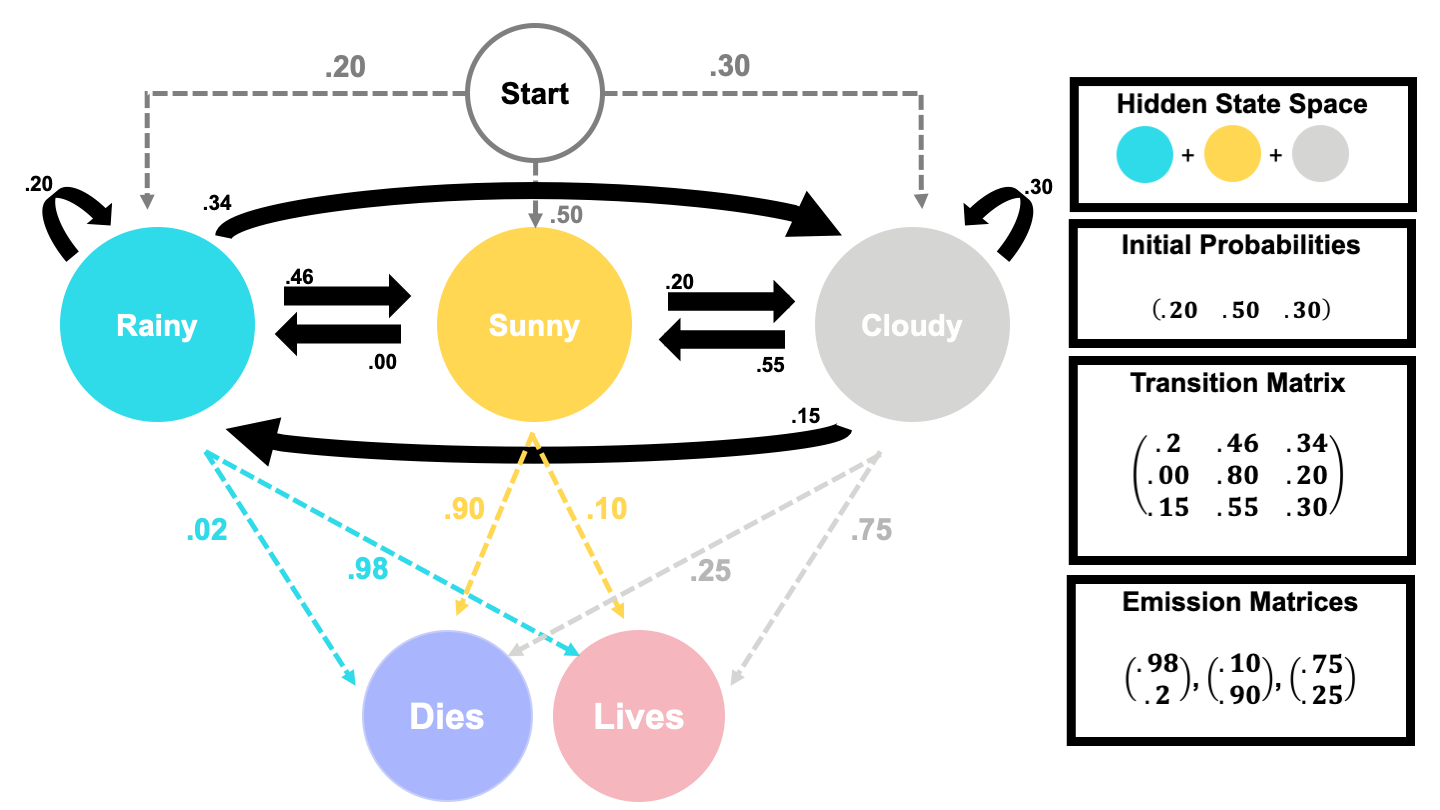
\includegraphics{images/HMM_Diagram_Frog.png}
\caption{Fig 2. HMM Directed Graph. Made by Author}
\end{figure}

\hfill\break

\textbf{Frog Animations}

We can reuse our previous animation to simulate state-space transitions and what that implies for our frog family's chance of living.

Now, the dots change colors with the true but unobserved weather of each day. Written text now describes,

\begin{itemize}
\tightlist
\item
  The emission probability of dying on a given day.
\item
  The number of unobserved, but true, weather states.
\end{itemize}

What a nice way of looking at the relationship between emission probabilities and the hidden states! In this next section, we'll see how we model the hidden states using observations.

\hfill\break

\begin{center}\rule{0.5\linewidth}{0.5pt}\end{center}

\hypertarget{algorithms}{%
\section{Algorithms}\label{algorithms}}

Let's say the frog family has been really lucky, and all the frogs who left the tree hide in the past week came back! One very curious frog named Betsy wonders what the probability of all her family surviving is, given the weather.

We can answer Betsy's questions using likelihood calculations or the Forward-Backward Algorithm.

\hypertarget{likelihood}{%
\subsection*{Likelihood}\label{likelihood}}
\addcontentsline{toc}{subsection}{Likelihood}

\textbf{Likelihood} or \textbf{Posterior Probability} are commonly defined as the probability of the data, given a true underlying parameter\footnote{\url{https://www.bayesrulesbook.com}}.

Let \(W_i\) be the hidden states of the weather in the past week, and let \(D_i\) be our observations on whether or not the frogs came back alive. This implies

\begin{align*}
W_i &= \{W_1= w_1, W_2=w_2, W_3=w_3,W_4= w_4, W_5=w_5, W_6=w_6, W_7=w_7\}\\
W_i &= \{w_1, w_2, w_3, w_4, w_5, w_6, w_7\} \\[15pt]
\text{and}\\[15pt]
D_i &= \{D_1= d_1, D_2=d_2, D_3=d_3,D_4= d_4, D_5=d_5, D_6=d_6, D_7=d_7\\
D_i &= \{d_1, d_2, d_3, d_4, d_5, d_6, d_7\}
\end{align*}

In this case, the likelihood would be the probability of our observed \(D_i\), given some true underlying set of \(W_i\). This is computed below.

\begin{align*}
P(D_i \mid W_i) &= P(d_1 \mid w_1)  \times  P(d_2 \mid w_2) \\ 
& \times  P(d_3 \mid w_3)  \times  P(d_4 \mid w_4) \\ &  \times  P(d_5 \mid w_5)  \times  P(d_6 \mid w_6) \\
& \times P(d_7 \mid w_7) \\
P(D_i \mid W_i) &= \prod_{i=1}^7 P(d_i \mid w_i)
\end{align*}

\begin{quote}
\textbf{NOTE:} The capital pi (\(\prod\)) means to multiply a series indexed by \(i\).
\end{quote}

\hfill\break

If we knew the states of the past week were \texttt{Sunny}, \texttt{Cloudy}, \texttt{Rainy}, \texttt{Rainy}, \texttt{Rainy}, \texttt{Rainy}, \texttt{Rainy} and everyone came back alive. We'd compute the likelihood as

\begin{align*}
P(D_i \mid W_i) &= P(Lives \mid Sunny) \times P(Lives \mid Cloudy)\\
&\times P(Lives \mid Rainy)\times P(Lives \mid Rainy) \\
&   \times P(Lives \mid Rainy) \times P(Lives \mid Rainy) \\
& \times P(Lives \mid Rainy) \\[10pt]
P(D_i \mid W_i) &= .10 \times .75 \times .98  \times .98  \times .98  \times .98  \times .98  \\
P(D_i \mid W_i) &= 0.06779406  \\
P(D_i \mid W_i) &\approx 0.068  \\
\end{align*}

\hfill\break

\textbf{Bad News:} We can't truly know the states of the \(W_i\)! Bummer.

Because of this, we would need to add together all likelihoods for all possible states for each event, weighted by their probability\footnote{\url{https://web.stanford.edu/~jurafsky/slp3/A.pdf}} . More succinctly, we intend to find the likelihood of all observations \(P(D_i)\), given the probability of all states \(P(D_i \cap W_i)\). We can do this with the rules of joint probability we covered in the previous section.

\begin{align*}
P(D_i \cap W_i) &= P(D_i \mid W_i)\times P(W_i) \\
&= \prod_{i=1}^7 P(d_i \mid w_i) \times P(W_i) && \text{by above}\\
&= \prod_{i=1}^7 P(d_i \mid w_i) \times \prod_{i=1}^7 P(w_i \mid w_{i-1}) && \text{by Markov}
\end{align*}

Now, we sum up all the observations given.

\[P(D_i) = \sum_{i=1}^n P(D_i \cap W_i) = \sum_{i=1}^n P(D_i \mid W_i)\times P(W_i)\]

So, for our 7 consecutive live frogs, this would be

\begin{align*}
P(D_i) &=P(Lives \mid Sunny) \times P(Lives \mid Sunny)\times P(Lives \mid Sunny)\\
&\times P(Lives \mid Sunny)\times P(Lives \mid Sunny)  \times P(Lives \mid Sunny)  \times P(Lives \mid Sunny) \\[10pt]
& + P(Lives \mid Cloudy) \times P(Lives \mid Sunny)\times P(Lives \mid Sunny)\\
&\times P(Lives \mid Sunny)\times P(Lives \mid Sunny)  \times P(Lives \mid Sunny) \times P(Lives \mid Sunny) \\[10pt]
& + P(Lives \mid Sunny) \times P(Lives \mid Cloudy)\times P(Lives \mid Sunny)\\
&\times P(Lives \mid Sunny)\times P(Lives \mid Sunny)  \times P(Lives \mid Sunny)  \times P(Lives \mid Sunny) \\[10pt]
& + P(Lives \mid Sunny) \times P(Lives \mid Sunny)\times P(Lives \mid Cloudy)\\
&\times P(Lives \mid Sunny)\times P(Lives \mid Sunny)  \times P(Lives \mid Sunny)  \times P(Lives \mid Sunny) \\[10pt]
&+ \dots \\[10pt]
&=P(Lives \mid Rainy) \times P(Lives \mid Rainy)\times P(Lives \mid Rainy)\\
&\times P(Lives \mid Rainy)\times P(Lives \mid Rainy)  \times P(Lives \mid Rainy)  \times P(Lives \mid Rainy) \\[10pt]
\end{align*}

That is \emph{extremely difficult} to do when we the number of our states (\(N\)) are numerous or we have some arbitrarily large number observations, \(T\), since we'd be analyzing \(N^T\) different possible sequences. However, we can predict the hidden states of HMMs like this one, using the Forward-Backward Algorithm.

\hypertarget{the-forward-backward-algorithm}{%
\subsection*{The Forward-Backward Algorithm}\label{the-forward-backward-algorithm}}
\addcontentsline{toc}{subsection}{The Forward-Backward Algorithm}

The Forward-Backward Algorithm is a dynamic programming algorithm used to infer the probability of seeing observations in a Hidden Markov Model. It contains two sub-algorithms, the Forward Algorithm \& the Backward Algorithm, which respectively compute the probability of the data from the beginning and the end of observations until they collide and result in a total probability of the data\footnote{\url{https://web.stanford.edu/~jurafsky/slp3/A.pdf}}. The process may seem extra, but as you've seen in the last section's toy computation, we have to be extra out of necessity.

\begin{quote}
\textbf{NOTE:} The following sections heavily drawn from the following sources \footnote{\url{https://web.stanford.edu/~jurafsky/slp3/A.pdf}} \footnote{\url{https://scholar.harvard.edu/files/adegirmenci/files/hmm_adegirmenci_2014.pdf}} \footnote{\url{https://www.cs.tut.fi/kurssit/SGN-24006/PDF/L08-HMMs.pdf}} \footnote{\url{http://www.columbia.edu/~mh2078/MachineLearningORFE/HMMs_MasterSlides.pdf}}
\end{quote}

\hypertarget{forward}{%
\subsubsection*{Forward}\label{forward}}
\addcontentsline{toc}{subsubsection}{Forward}

In the first section of the Forward-Backward Algorithm, we compute the \textbf{forward probabilities}. Forward probabilities are informally the joint probability of all observations so far and the probability of being in some given state space.

Formally, a forward probability is defined as
\[\alpha_k(j) = P(d_1, \dots , d_k,w_k = j \mid \mathbb{F}) \]
\textgreater{} \textbf{NOTE:} That is, we compute the probability of the first \(k\) observations (\(d_1,\dots, d_k\)) leading us to our current observation while also being in state \(j\), \(\alpha_k(j)\).

To compute the forward probabilities, we must

\begin{itemize}
\tightlist
\item
  Sum over all previous forward probabilities that would lead us to be in \(\alpha_k(j)\)
\item
  Multiply by the transition probabilities \(\mathbb{a}_{ij}\) describing the change from the previous state \(i\) to the current state \(j\).
\item
  Multiply again by the emission probabilities of our current observation \(d_k\), given the state \(j\). That is \(b_j(d_{k})\).
\end{itemize}

Formally, this is written as

\[\alpha_{k}(j) = \left[\sum_{i=1}^\mathbb{W} \alpha_{k-1}(i) \mathbb{a}_{ij} \right]b_j(w_{k})\]

\begin{quote}
\textbf{Note:} Remember that \(\mathbb{W}\) is the state space!
\end{quote}

\hfill\break

In practice, we typically use recursion to compute the probability of our observations. Like so

1.) \textbf{Base Case:} We use the initial probability of our system's states.

\begin{align*}
\alpha_1(j) = \pi_jb_j(d_1) && \text{for } 1 \leq j \leq \mathbb{W}
\end{align*}

2.) \textbf{Recursion:} We use the previous case \& transition \& emission probabilities to compute the probability of being in the newest state \(j\).

\begin{align*}
\alpha_{k}(j) = \left[\sum_{i=1}^\mathbb{W} \alpha_{k-1}(i) \mathbb{a}_{ij} \right]b_j(d_{k}) && \text{for } 1 \leq j \leq \mathbb{W}, 1 \leq k \leq n
\end{align*}

2.) \textbf{End:} We can then define the probability of the observations as the recursive sum of all forward probabilities.

\[P(D_{1:n} = d_{1:n} \mid \lambda) = \sum_{i=1}^\mathbb{W} \alpha_{n}(i)\]

\hypertarget{backward}{%
\subsubsection*{Backward}\label{backward}}
\addcontentsline{toc}{subsubsection}{Backward}

In the second section of the Forward-Backward Algorithm, we compute the \textbf{backward probabilities}. Backward probabilities are informally the joint probability of successive observations and the probability of being in some arbitrary state \(v\), given that we start an observation \(k+1\).

Formally, a backward probability is defined as
\[\beta_k(v) = P(d_{k+1}, \dots , d_n, \mid w_k = v , \mathbb{F}) \]

To compute the backward probabilities, we must
- Sum the successive values after \(\beta_{k+1}\) until the end of the k-observations at \(d_n\).
- Multiply by the transition probabilities \(\mathbb{a}_{vj}\) describing the change from the given current state \(v\) to the next state \(j\).
- Multiply again by the emission probabilities of the success observation \(d_{k+1}\). That is \(b_j(d_{k+1})\).

Formally, this is written as

\[\beta_k(v) = \sum_{j=1}^\mathbb{W} \mathbb{a}_{vj}b_j(d_{k+1}) \beta_{k+1}(j) \]

\begin{quote}
\textbf{Note:} Remember that \(\mathbb{W}\) is the state space!
\end{quote}

\hfill\break

In practice, we typically use recursion to compute the probability of our observations. Like so

1.) \textbf{Base Case:} We use the initial probability of our system's states. The value is 1 since we're working backward!

\begin{align*}
\beta_n(i) = 1 && \text{for } 1 \leq v \leq \mathbb{W}
\end{align*}

2.) \textbf{Recursion:} We use the previous transition \& emission probabilities of being in the previous state \(i\) from the state \(j\) to weigh the sum of all success values.

\begin{align*}
\beta_k(v) = \sum_{j=1}^\mathbb{W} \mathbb{a}_{vj}b_j(d_{k+1}) \beta_{k+1}(j) && \text{for } 1 \leq v \leq \mathbb{W}, 1 \leq k \leq n
\end{align*}

2.) \textbf{End:} We can then define the backward probability of the observations as the recursive sum of values after \(k\), beginning with the end value.

\[P(D_{k+1:n} =d_{k+1:n} \mid \lambda) = \sum^\mathbb{W}_{j=1}\pi_j b_j(d_1)\beta_1(j)\]
In the end, we've done the same thing! But now, we can use the probabilities of our observations to study the distribution of the hidden states.

\hypertarget{collision}{%
\subsubsection*{Collision}\label{collision}}
\addcontentsline{toc}{subsubsection}{Collision}

We can use Bayes' Rule, joint probability, and our previous work to compute the probability of being in a state \(v\) at a given time, \(t\). This is commonly called a \textbf{smoother} analysis. Like before, we will use the notation of our frog example to describe the states (\(W_i\)) and observations (\(D_i\)).

By Bayes' Rule, the probability of being in state, \(v\), given the observations, is

\[\gamma_t(v) =  P(W_t = v \mid D_i) = \frac{P(W_i \cap D_i )}{P(D_i)} \]

However, we can make this simpler by acknowledging that \(P(W_i \mid D_i)\) is proportional (e.g., division by a constant value) to the joint probability of \(W_i\) and \(D_i\). So,

\begin{align*}
\gamma_t(v)  &\propto P(W_i \cap D_i) \\
\end{align*}

We can simplify this even further by splitting our \(n\) observations at the \(k^th\) observation, like

\begin{itemize}
\tightlist
\item
  \(D_{i} = \{d_1, \dots, d_n\}\)
\item
  \(D_{1:k} = \{d_1, \dots, d_k\}\)
\item
  \(D_{k+1:n} = \{d_{k+1}, \dots, d_{n}\}\)
\end{itemize}

Then,

\begin{align*}
\gamma_t(v)  &\propto P(W_i \cap D_i) \\
&\propto P(D_{k+1:n} \mid W_i \cap D_{1:k}) \times P(W_i  \cap D_{1:k}) && \text{by Bayes Rule}\\
&\propto P(D_{k+1:n} \mid W_i) \times P(W_i  \cap D_{1:k}) && \text{by Markov Property of } D_i\\
\end{align*}

We recognize these as the backward probability times the forward. We include our constant value \(\frac{1}{ \sum^\mathbb{W}\beta_t(v) \times \alpha_t(v)}\).

\begin{align*}
\gamma_t(v) =  P(W_t = v \mid D_i) = \text{backward} \times \text{forward} \times \frac{1}{ \sum^\mathbb{W} \beta_t(v) \times \alpha_t(v)}
\end{align*}

\begin{quote}
\textbf{Note:} We've multiplied by the constant value of \(\frac{1}{ \sum^\mathbb{W}\beta_t(v) \times \alpha_t(v)}\) because the marginal distribution of the \(D_i\) would be the sum of the probabilities of the observations for each possible state, by the Law of Total Probability.
\end{quote}

Thus, the probability of being in a given state \(v\), at a particular time, \(t\), given the data is

\[\gamma_t(v) =  P(W_t = v \mid D_i) = \frac{\beta_t(v) \times \alpha_t(v)}{\sum^\mathbb{W} \beta_t(v) \times \alpha_t(v)}\]

We did it! Intuitively, it might not make sense why we can compute the probability of being at a state by multiplying the backward \& forward probabilities, then dividing by the possible states.

The idea is that the recursive functions ``scan'' through the observations, determining some probability of the next or previous outcome, until they \emph{collide} and essentially collapse onto a probability of that observation. They do this for each possible observation. Then, by dividing the total probability of the observations, we can get the probability of the \(v\)-state.

\hypertarget{conclusion-1}{%
\section{Conclusion}\label{conclusion-1}}

We did it! We've learned how to compute the probability of the observations \& the probability of a particular state, given a time, using the Forward-Backward Algorithm. There are, of course, other problems that Hidden Markov Models can solve, like finding the most probable sequence of \emph{all} states or how to maximize the functions forward or backward functions.

However, the Forward-Backward Algorithm has \emph{so} many meaningful applications throughout the natural \& social sciences alone. We'll look at a couple in the next chapter.

If you have any lingering questions, I've linked some great YouTube videos that may be helpful below.

\hypertarget{video-resources-1}{%
\section*{Video Resources}\label{video-resources-1}}
\addcontentsline{toc}{section}{Video Resources}

\textbf{Hidden Markov Model Properties}

\textbf{Forward Backward \& Likelihood}

\hfill\break

\hypertarget{references-1}{%
\section*{References}\label{references-1}}
\addcontentsline{toc}{section}{References}

\hypertarget{application-to-statistical-genetics}{%
\chapter{Application to Statistical Genetics}\label{application-to-statistical-genetics}}

The goals of epidemiology explicitly revolve around studying the incidence, distribution, and control of disease. As one can imagine, the boundaries of the field are highly nebulous. So far, we've looked at Hidden Markov Models as mathematical objects devoid of any real context--- aside from a toy frog example. This section intends to tie together the mathematical principles of HMMs with their connections to big areas in biostatistical \& epidemiological research. We find that, yes, HMMs \emph{are} cool because they can help save lives, bridge the gaps across survival disparities, and study our bodies.

\hfill\break

\begin{center}\rule{0.5\linewidth}{0.5pt}\end{center}

\hypertarget{local-ancestry-inference}{%
\section{Local Ancestry Inference}\label{local-ancestry-inference}}

Local Ancestry Inference (LAI) is an approach in statistical genetics \& bioinformatics that aims to study genetic diversity, disease prevalence, or evolutionary development by linking each segment of a genome to some ancestral population\footnote{\url{http://cs229.stanford.edu/proj2015/290_report.pdf}}. LAI has been used to study crop plant analysis\footnote{\url{https://www.ncbi.nlm.nih.gov/pmc/articles/PMC7003078/}}, Tilapia breeding\footnote{\url{https://www.nature.com/articles/s41598-020-75744-9}}, and the genetic adaptations of cows in East Africa\footnote{\url{https://www.frontiersin.org/articles/10.3389/fgene.2014.00443/full}}. However, using LAI in public health studies is a critically important step when studying ethnically diverse cohorts.

Diasporic movement, mass migration, colonial empire, and slavery have profoundly changed the genetic landscape of the human population. Prior to these \emph{admixture events}, human communities were largely isolated from each other, and over time, these isolated communities genetically diverged into human sub-populations. The differences between sub-populations are largely minuscule. While the differences are mostly nonexistent, generations of independent breeding did allow for the development of genes \& mutations that are more common in some sub-populations rather than others\footnote{\url{https://pubmed.ncbi.nlm.nih.gov/20594047/}}.

\begin{quote}
\textbf{NOTE:} Ancestry \& Race are two different concepts that do not measure the same thing in the same way.
\end{quote}

Admixed populations are products of the intense migratory \& diasporic events that marked the 14th-19th centuries, which resulted in populations whose genetic ancestries were from 2 or more human sub-populations. We call these ancestrally-mixed populations \textbf{admixed} populations. Notable examples of admixed populations include African Americans, Latines, Ashkenazi Jews, and SWANA peoples. However, admixture is everpresent across most global populations. For example, this plot made by Hodgson et al.~shows the admixture proportion across 81 different African populations with colorings for 10, 11, and 12 respective common ancestries \footnote{\url{http://journals.plos.org/plosgenetics/article?id=10.1371/journal.pgen.1004393}}.

\hfill\break

\begin{figure}
\centering
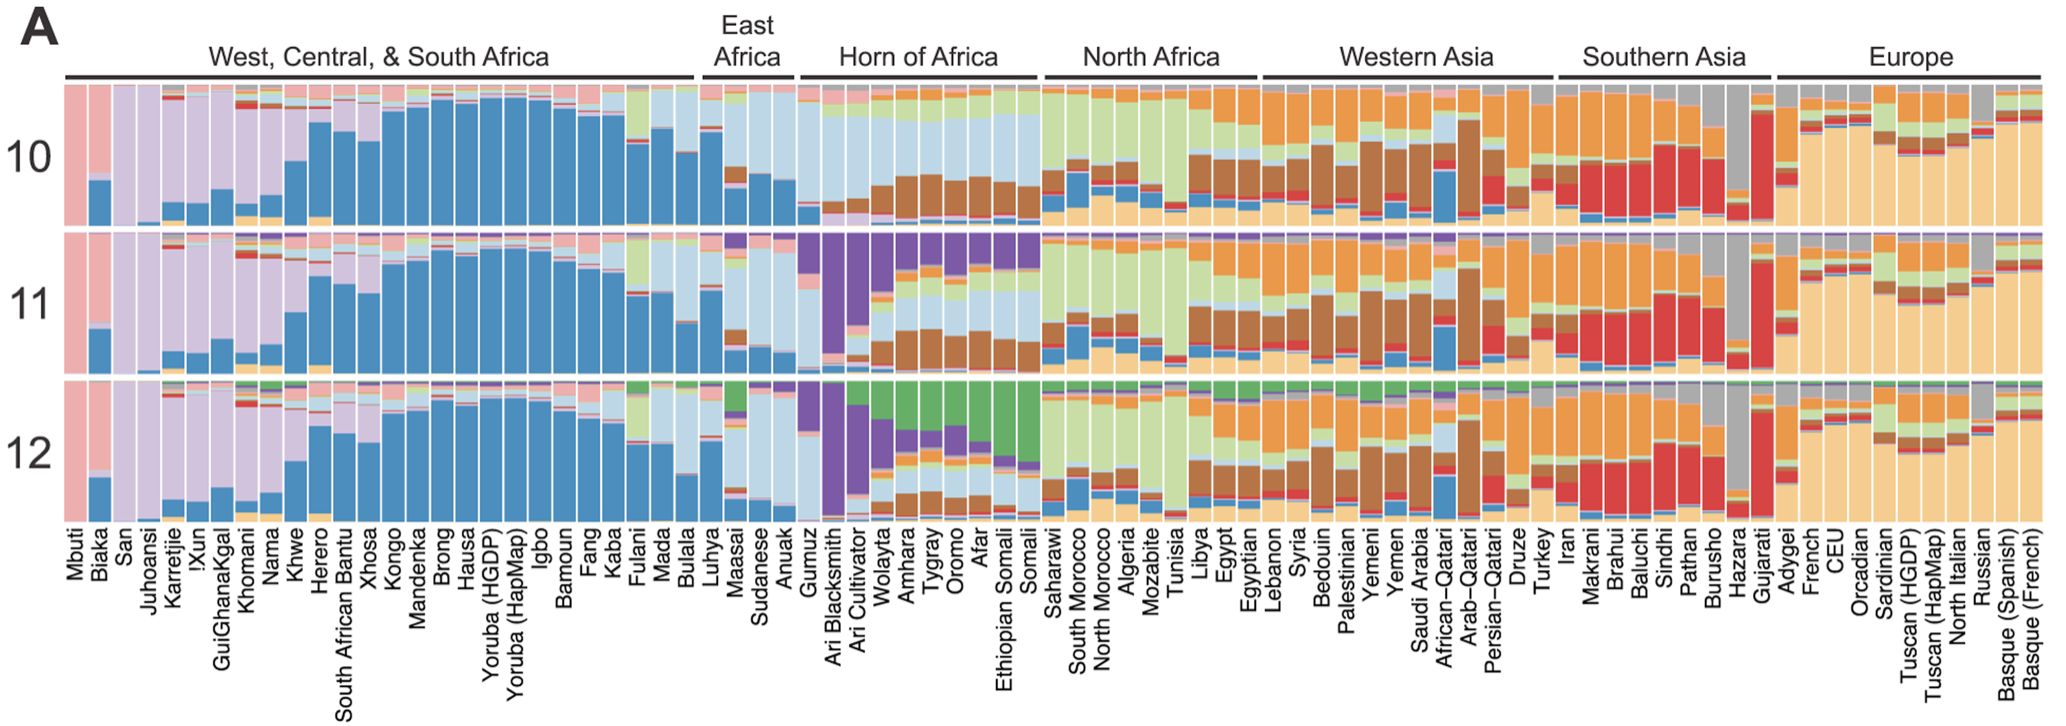
\includegraphics{images/map.png}
\caption{Figure 1. Admixture proportions of Horn of Africa populations (Hodgson et al.)}
\end{figure}

\hfill\break

Unfortunately, the violence of diaspora, colonialism, and enslavement also brought the dangers of inheriting potentially dangerous mutations by family, ancestry, or ethnicity. For example, the inheritance of Tay-Sachs, Ellis-van Creveld Syndrome, diabetes, and prostate cancer all occur with strong associations to ancestry\footnote{\url{https://pubmed.ncbi.nlm.nih.gov/20594047/}}.

So, when studying disease with evidence of some ancestral association, LAI allows public researchers to first map the ancestry of an individual's genome, before going on to find associations between disease \& ancestral lineage.

\hypertarget{local-ancestry}{%
\subsection*{Local Ancestry}\label{local-ancestry}}
\addcontentsline{toc}{subsection}{Local Ancestry}

Local Ancestry is formally defined as ``the genetic ancestry of an individual at a particular chromosomal location, where an individual can have 0, 1, or 2 copies of an allele derived from each ancestral population.\footnote{\url{https://onlinelibrary.wiley.com/doi/abs/10.1002/gepi.21819}}''

Due to the structure of gene inheritance, we can model local ancestry as a Hidden Markov Model, with the observed! This idea has been formalized throughout the literature on statistical genetics, but we will look at one particular approach of using HMMs in the software HAPMIX to infer local ancestry in admixed populations.

\hypertarget{hapmix}{%
\subsection*{HAPMIX}\label{hapmix}}
\addcontentsline{toc}{subsection}{HAPMIX}

\begin{quote}
\textbf{NOTE:} Most content in this section originates from HAPMIX's official release paper by Price et al.\footnote{\url{https://journals.plos.org/plosgenetics/article?id=10.1371/journal.pgen.1000519}}.
\end{quote}

\textbf{Definitions}

\begin{itemize}
\tightlist
\item
  A haplotype is a gene that is solely inherited from one parent and thus one parental population. Haplotypes are generally considered good markers of ancestral lineage.
\end{itemize}

\textbf{Assumptions:}

\begin{itemize}
\tightlist
\item
  We assume that the admixed population comes from only two ancestral populations
\item
  We have access to reference data derived from unadmixed reference populations
\item
  The unadmixed reference populations are closely related to the true ancestral populations.
\end{itemize}

\textbf{Process}

\begin{enumerate}
\def\labelenumi{\arabic{enumi})}
\item
  At every locus, HAPMIX estimates the likelihood that a ``parental'' haplotype from an admixed individual comes from a referenced ancestral population.
\item
  Loci that are next to each other are more likely to come from the same ancestral lineage\footnote{due to a concept called Linkage Disequilibrium}, but that doesn't hold true after enough positions. So, we say that the number of genes inherited from an ancestral population at the \(j^th\) locus can be strictly predicted by the ancestry of the \({j-1}^{th}\) locus.
\item
  We can then use an HMM where the hidden states are the number of ancestral genes inherited \((0,1,2)\) at locus \(j\), and the observations are the likelihoods of observing some mutation at locus \(j\), given the ancestral reference panel.
\item
  Using a smoother analysis, similar to the Forward-Backward Algorithm, we can combine these likelihoods to provide a probabilistic estimate of ancestry at each locus.
\end{enumerate}

\textbf{Visual}

Below is a visual made by Price et al.~describing the HMM employed in HAPMIX.

\begin{figure}
\centering
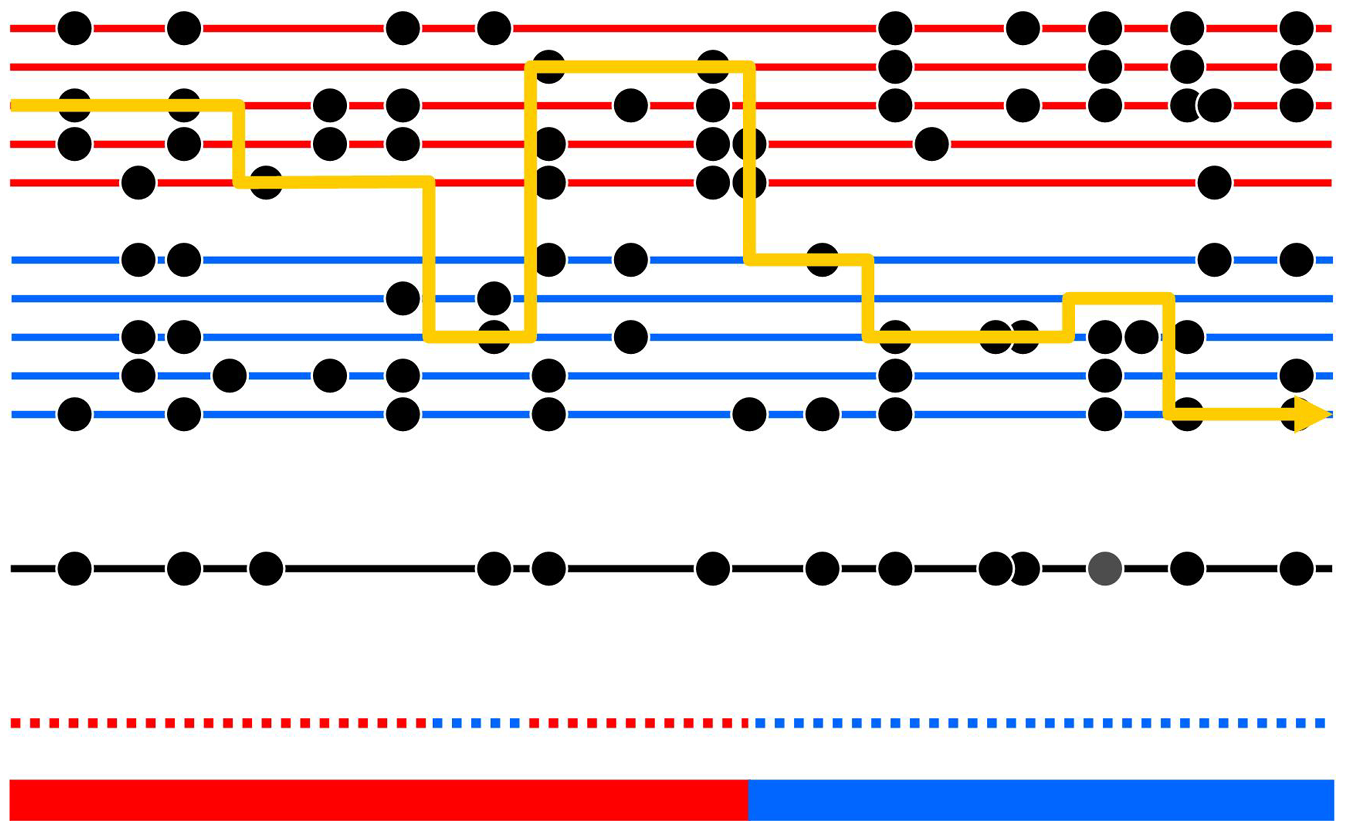
\includegraphics{images/hapmix.png}
\caption{Fig 2. Markov Schematic (Price et al.)}
\end{figure}

\begin{itemize}
\tightlist
\item
  The thick bottom bar represents the true 2-state ancestral composition of an individual, and the dotted line above it represents the ancestral reference panel, from which we compute likelihoods.
\item
  The line line represents a chromosomal segment of an individual, while the black circles represent typed mutations sites that can be distinguished between the ancestries.
\item
  When the yellow line crosses a red or blue line, it is visualizing the selection of an ancestral group, given the individual's observed chromosome. Notice that when the line crosses through a dot on one particular side, it will choose the side with equal or greater dots that are vertically aligned.
\item
  The yellow line can misclassify the ancestries since this is a probabilistic model. Notice the portion of blue dots above the red bar.
\end{itemize}

\hypertarget{conclusion-2}{%
\subsection{Conclusion}\label{conclusion-2}}

LAI is only one application of HMMs. Variations of HMMs can be used to study the differential use of condoms for HIV prevention\footnote{\url{https://www.ncbi.nlm.nih.gov/pmc/articles/PMC3649016/}}, the race-differences in the progression of HIV for vulnerable, infected, and AIDS positive people between African American \& White People\footnote{\url{https://www.ncbi.nlm.nih.gov/pmc/articles/PMC4023279/}}, or even when automatically monitoring the development of Influenza outbreaks\footnote{\url{https://link.springer.com/chapter/10.1007/978-3-540-45231-7_48}}.

This is only a primer (with a de-emphasis on application), but I absolutely suggest reading through the footnote references to so how cool HMMs become when using them to find ways of helping people, treating illness, and more!

\hfill\break

\hypertarget{references-2}{%
\section*{References}\label{references-2}}
\addcontentsline{toc}{section}{References}

  \bibliography{book.bib,packages.bib}

\end{document}
